\section{Results and Discussion}
\label{sec:methodology}

% QC score rewards if drug and disease genes are placed in the same cluster, no penalty if not


% TODO
% disease-disease lists drugs with two common drugs per row: Drug - Disease of Interest - other Disease -> Visualize BIPARTITE GRAPH (not that relevant for me)

% find smth that could be related to target disease
% org med indication -> paper that relates drug to some mechanism
% -¨- -> look at most represented onLabel disease

% ==> try to find out if prediction could make sense

\subsection{Predicted repurposable drugs for COVID-19}

Table \ref{tab:predDrugsCovid} shows the first 20 drugs predicted by SAveRUNNER for COVID-19 sorted by the associated p-values in ascending order. In total 101 repurposable drugs were predicted for COVID-19.

\begin{table}[H]
\begin{center}
%\parbox{11cm}{
\captionsetup{width=10.5cm}
\caption{Predicted repurposable drugs for COVID-19. Values are sorted by p-values and are also rounded to three decimals. Only the drugs with 20 lowest p values are shown.}
\label{tab:predDrugsCovid}
%}
\npdecimalsign{.}
\begin{tabular}{ l S S }
    \toprule
    \text{Drug} & \text{p-Value} & \text{Adjusted Similarity} \\
    \midrule
azacitidine     & 1.698e-07 & 1.000e+00             \\
riboflavin      & 1.910e-06 & 9.932e-01             \\
noscapine       & 9.400e-06 & 1.000e+00             \\
phylloquinone   & 1.288e-05 & 9.994e-01             \\
flavin adenine dinucleotide & 4.693e-05 & 9.631e-01 \\
decitabine      & 9.737e-05 & 1.000e+00             \\
isoniazid       & 1.047e-04 & 9.932e-01             \\
tadalafil       & 1.064e-04 & 9.932e-01             \\
avanafil        & 1.373e-04 & 9.932e-01             \\
latanoprost     & 1.435e-04 & 9.932e-01             \\
telotristat ethyl & 4.260e-04 & 9.932e-01           \\
kappadione      & 5.929e-04 & 9.967e-01             \\
sapropterin     & 7.441e-04 & 9.932e-01             \\
ixekizumab      & 7.785e-04 & 9.932e-01             \\
menadione       & 8.224e-04 & 9.856e-01             \\
anisindione     & 1.231e-03 & 1.000e+00             \\
roflumilast     & 1.361e-03 & 9.932e-01             \\
papaverine      & 1.378e-03 & 9.932e-01             \\
acrivastine     & 1.418e-03 & 9.932e-01             \\
flucytosine     & 2.170e-03 & 1.000e+00             \\

\bottomrule
\end{tabular}
\npnoround

\end{center}
\end{table}

For the drug with the lowest p-value, Azacitidine, there is at least one reported case where this drug was involved in the successful treatment of COVID-19 \cite{Taurino_2021}. However, this patient also suffered from pneumonia and concurrent acute myeloid leukemia, which is one of the target diseases of Azacitidine \cite{Wishart2017}. It is questionable how much impact Azacitidine had in defense against SARS-CoV-2. Despite that, the results from SAveRUNNER makes this case worth investigating.\\
Next on table \ref{tab:predDrugsCovid} is Riboflavin, which is a vitamin to correct vitamin B2 deficiency \cite{Wishart2017}. Multiple publications report a positive effect of Riboflavin in combination with UV light regarding the concentration of SARS-CoV-2 in liquid samples (blood or plasma) \cite{Ragan_2020, Yonemura_2021}. \\
Noscapine, the drug with the 3rd lowest p-value, is used against the common cold, coughs and respiratory diseases \cite{Wishart2017}. These symptoms are some of the most common symptoms found in COVID-19 patients, hence it appears worth investigating whether the symptomatic treatment increases the recovery rate of patients. \\
Phylloquinone appears to be the generic name for Vitamin K1. Not much information is available on K1 in regards to COVID-19. However, two investigations note the connection to the so-called endothelial protein S which appears to be able to prevent the cytokine storm observed in COVID-19 cases \cite{Popa_2021, Dofferhoff_2020}. Furthermore, vitamin K depletion has been reported in COVID-19 patients \cite{Dofferhoff_2020}. This suggests that administration of this vitamin may allow to lessen the severity or prevent the cytokine storm. This over-reaction of the immune system occurs during the most severe stage of the disease. If it could be lessened, the already weakened patients may have higher chances of survival.


% --------------------------------------------------------------------------------

\subsection{Matched on-Label diseases of predicted drugs}

Figure \ref{fig:onLabel} shows the original (on-label) targets for the predicted drugs, according to the therapeutic drug database \cite{Zhou_2022}, which may be interesting for several reasons. For once, on-label and off-label diseases might share a certain characteristic, symptoms for example. This might then help to further explain the repurposability of a certain drug or group of drugs.
Furthermore, the proximity of the on-label and off-label disease modules in the underlying protein interactome can potentially be reflected in such an analysis as well.

\begin{figure}[H]
    \captionsetup{width=0.7\textwidth}
    \centering
    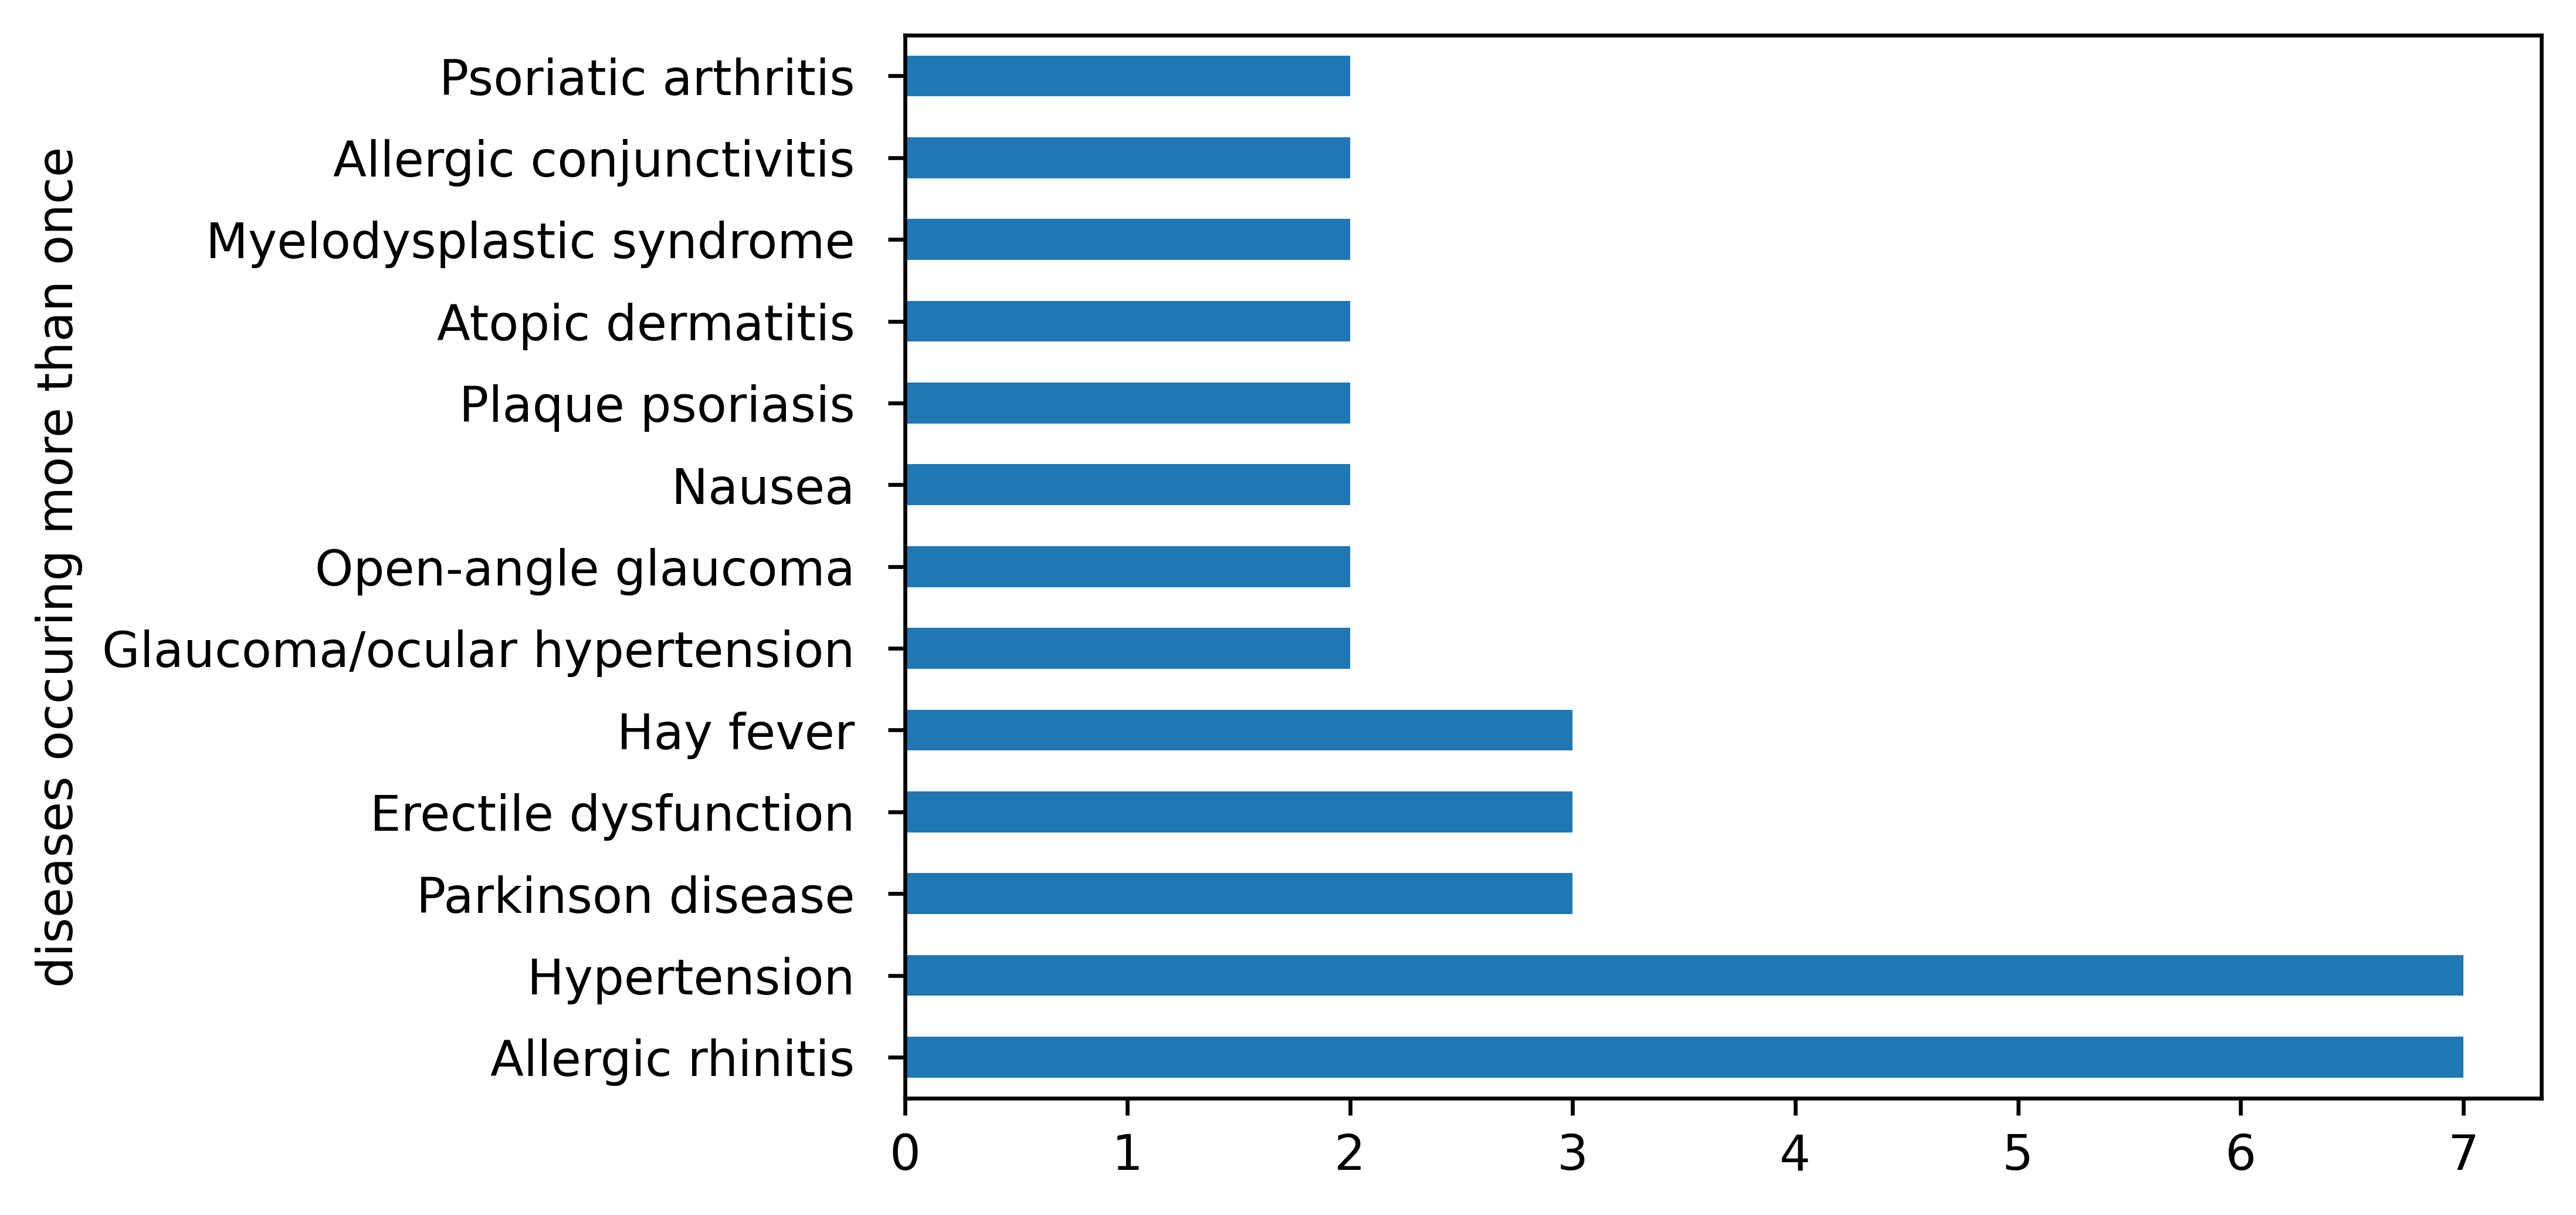
\includegraphics[width=0.7\textwidth]{figures/onLabel_diseases_saverunner_covid.png}
    \caption{On Label targets for drugs predicted by SAveRUNNER that occur more than once.}
    \label{fig:onLabel}
\end{figure}

Some of the hypertension-related drugs will be investigated in the next section. These three as well as deserpidine and Perindopril all affect the ACE protein, which is vital in the infection process of SARS-CoV-2. Another drug in this group, verapamil, does not affect ACE according to the DrugBank \cite{Wishart2017}. However, the adjusted similarity for this drug is also lower than for the ACE-inhibiting drugs. This drug is either not beneficial for the treatment of COVID-19 after all (but still close enough to the disease module in the interactome) or is potentially useful in another way. This would require further investigations.
The drugs associated with Allergic rhinitis are more difficult to link to COVID-19. Methdilazine, Clemastine, Cetirizine, and Fexofenadine all interact with H1 histamine receptor or act as antagonists to histamine $H_{1}$ \cite{Wishart2017}. As SARS-CoV-2 interacts with different parts of the immune system, these drugs' targets might be close enough in the network to lead to positive results by SAveRUNNER. Whether there is an actual molecular benefit for COVID-19 treatment needs to be investigated as well. Interestingly two publications investigating drugs related to histamine H2 receptor could not find any benefits for treatment of COVID-19 or suggested monitoring of patients during treatment with these drugs due to severe adverse effects \cite{Kim_2021, Chiu_2021}. Whether this translates to having similar effects for the H1 histamine receptor is uncertain.

% --------------------------------------------------------------------------------

\newpage
\subsection{Overlap with SARS}

Since SARS-CoV-2 has a genome sequence that is 75–80\% identical to that of SARS-CoV-1, it makes sense to look at drugs that could be used for both diseases \cite{Ghasemnejad_Berenji_2020}. Multi-target therapeutic agents have other benefits. Those can be better predictive pharmacokinetics, better patient compliance and reduced risk of drug interactions \cite{Mohamed_2021}.\\
Figure \ref{fig:Network} presents the Drug-Disease network for SARS and COVID-19. An edge is drawn between a drug (circular node) and a disease (rectangular) if SAveRUNNER predicted this drug as repurposable for this disease. Hence, the drug nodes a colored respective to the diseases for which they have a higher adjusted similarity (green - SARS; blue - COVID-19). The color of edges reflects the adjusted Similarity as well, where yellow corresponds to a high and blue to a low adjusted similarity. The force-directed graph layout of nodes tries to minimize overlapping nodes and crossing edges. 
This visualization is not ideal, as not all details are well visible. Still some characteristics of this network are noticeable. For once it appears that only a few drugs have a high adjusted similarity to both SARS and COVID-19. Most of the nodes that are predicted as repurposable for both diseases have a higher adjusted similarity to COVID-19. 
Furthermore, it is noticeable that some predicted drugs only have low adjusted similarity to SARS but no connection to COVID-19 at all. Meanwhile, this does not seem to occur for drugs associated with COVID-19 at all. 
Lastly, the amount of drugs associated with just COVID-19 seems much lower. A reason for this could be, that there are simply fewer data available as the first occurrence of COVID-19 is much more recent.  \\
Figure \ref{fig:DrugDiesease} illustrates that most drugs only have high adjusted similarity for either of the analyzed diseases. This means that finding a drug that can be used equally well to treat both diseases will be unlikely. Furthermore, the clustering separates the drugs well by their adjusted similarity, forming one cluster per disease on the highest level. \\
Figure \ref{fig:DieseaseDiesease} shows the Hamming Distance between each disease. There are 50 diseases that have been predicted for both COVID-19 and SARS by SAveRUNNER. These are candidates that are especially interesting as the immediate re-applicability can further help reduce the time and cost required for disease-specific testing.

\begin{figure}[H]
     \centering
    \begin{subfigure}{\textwidth}%[H]
        \captionsetup{width=\textwidth}
        \centering
        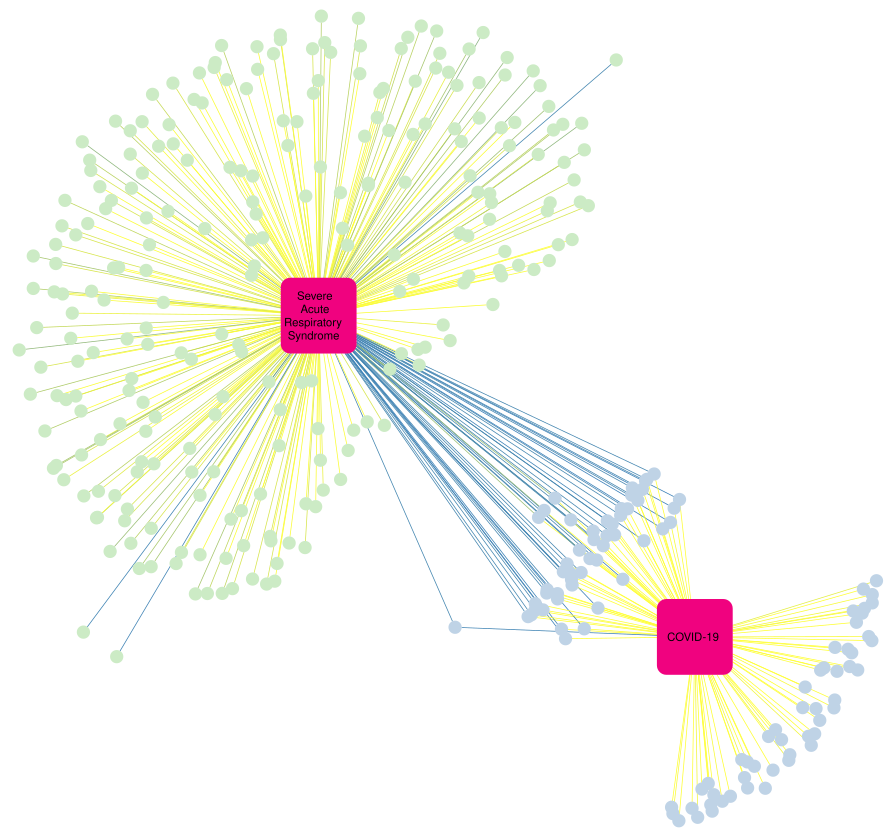
\includegraphics[width=\textwidth]{figures/COVID19xSARS_network.png}
        \caption{Network visualizing predicted repurposable drugs for COVID-19 and SARS. Yellow edges indicate a high adjusted similarity for the connected disease, while blue indicates a low value. Repurposable drugs associated with SARS are colored in green and drugs associated with COVID-19 are colored in blue.}
        \label{fig:Network}
    \end{subfigure}
     \hfill
     \begin{subfigure}[b]{0.45\textwidth}
         \centering
         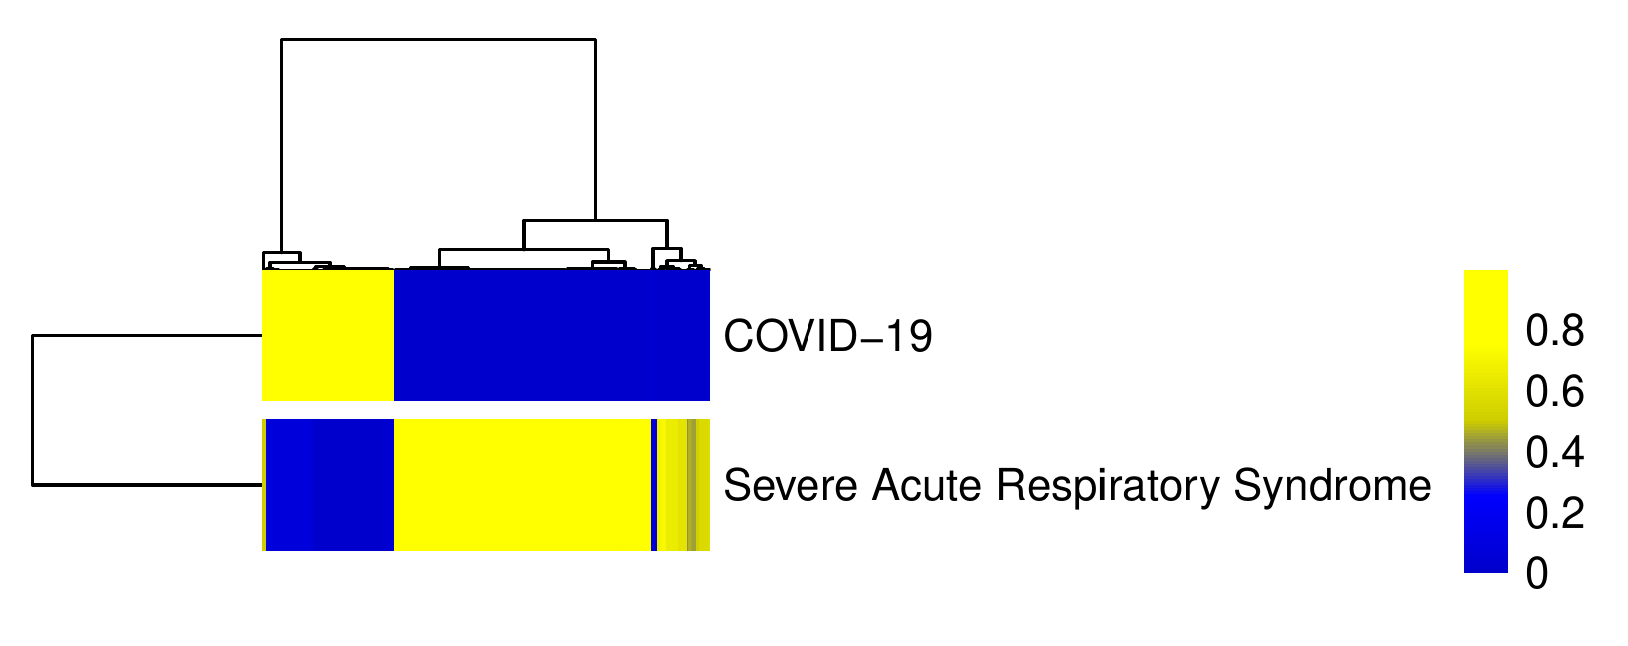
\includegraphics[width=\textwidth]{figures/Disease_Drug_Heatmap.png}
         \caption{Clusterd heatmap visualizing the adjusted similarity of both diseases per Drug. The color map ranges from blue (low) to yellow (high)}
         \label{fig:DrugDiesease}
     \end{subfigure}
     \hfill
     \begin{subfigure}[b]{0.45\textwidth}
         \centering
         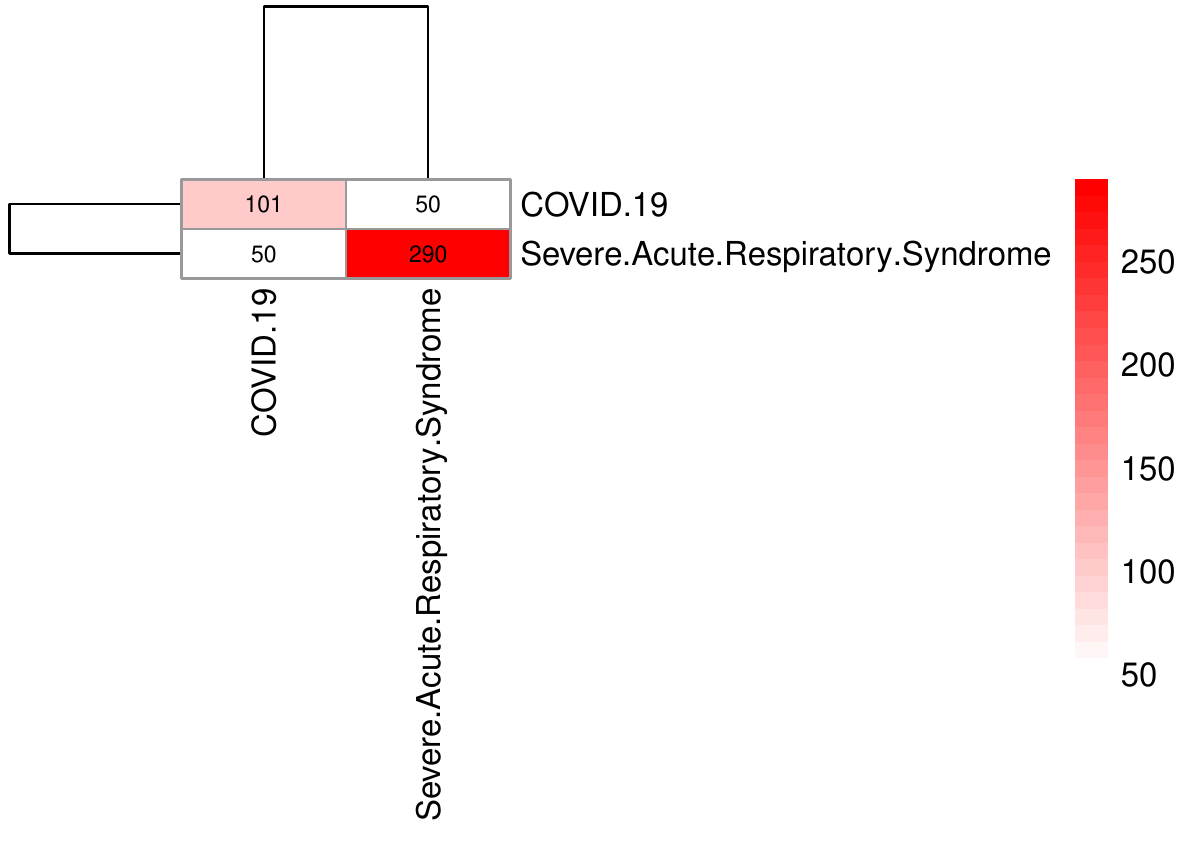
\includegraphics[width=\textwidth]{figures/Disease_Disease_Heatmap.png}
         \caption{clustered heatmap visualizing amount of shared  drugs between diseases.}
         \label{fig:DieseaseDiesease}
     \end{subfigure}
        \caption{Comparison of predicted repurposable drugs for COVID-19 and SARS.}
        \label{fig:SARS_COVID}
\end{figure}

The most notable drugs from this view are the ones that are shared and have high adjusted similarity for both diseases. The drugs for which this is the case are shown below. Table \ref{fig:predDrugsShared} shows the individual adjusted similarities per disease as well as the sum per drug.

\begin{table}[H]
\begin{center}

\captionsetup{width=9cm}
\caption{Predicted Drugs for both SARS and COVID-19 with the highest summed adjusted similarity for to both diseases. [\ref{sec:appendix}]}
\label{fig:predDrugsShared}

\npdecimalsign{.}
\nprounddigits{3}
\begin{tabular}{ l n{2}{5} n{2}{5} n{2}{5}}
    \toprule
    \text{Drug} & \text{COVID-19} & \text{SARS} & \text{Sum} \\
    \midrule
    \text{benazepril}  & 0.9932432669830258 & 0.504781792120694 & 1.4980250591037199  \\
    \text{cilazapril} & 0.9932432669830258 & 0.504781792120694 & 1.4980250591037199  \\
    \text{quinapril} & 0.9932432669830258 & 0.504781792120694 & 1.4980250591037199  \\
    \text{turoctocog alfa pegol} & 0.9932432669830258 & 0.161441849724981   & 1.1546851167080068 \\
    \bottomrule
\end{tabular}
\npnoround

\end{center}
\end{table}

The tabular data makes it clear that the drugs that have been predicted for both diseases are below non-shared drugs in similarity. However, the chance that these drugs might be repurposable for both diseases, makes the investigation worthwhile. 
All of the top 3 drugs shown in Table \ref{fig:predDrugsShared} share one interesting target \cite{Wishart2017}. This target is the aforementioned Angiotensin-converting enzyme (ACE). As stated above the ACE2 protein is required in order to allow the virus to enter the host cell. All three drugs act as inhibitors of ACE and are originally used for hypertension and heart failure \cite{Wishart2017}. Perhaps, this inhibition also prevents membrane fusion to be triggered by the virus.
The last drug of this subselection is Turoctocog alfa pegol. It is intended to be used to reduce the frequency and severity of bleeding episodes in Haemophilia patients \cite{Wishart2017}. Why this drug was predicted to be useful against COVID-19 and SARS requires further investigation.

% --------------------------------------------------------------------------------

